% ---------------------------------------------------------------
% Generated by Flowchart -> TikZ Studio
% Every coordinate below is derived from the editor diagram model.
% Safe to edit by hand, but regenerating will overwrite changes.
% ---------------------------------------------------------------

\documentclass[border=8pt]{standalone}
\usepackage[T1]{fontenc}
\usepackage[utf8]{inputenc}
\usepackage{xcolor}
\usepackage{tikz}
\usetikzlibrary{shapes.geometric,shapes.misc}

% ---- Colour definitions ----
\definecolor{fc12161C}{HTML}{12161C}
\definecolor{fc1F2933}{HTML}{1F2933}

% ---- Style definitions ----
\tikzset{
  fcnode/.style={
    draw, inner sep=0pt, outer sep=0pt, align=center,
    line join=round, line cap=butt
  },
  fcpath/.style={line join=round, line cap=butt},
  fcedge/.style={line join=round, line cap=butt},
  fclabel/.style={inner sep=1.4pt, outer sep=0pt, align=center},
}

\begin{document}
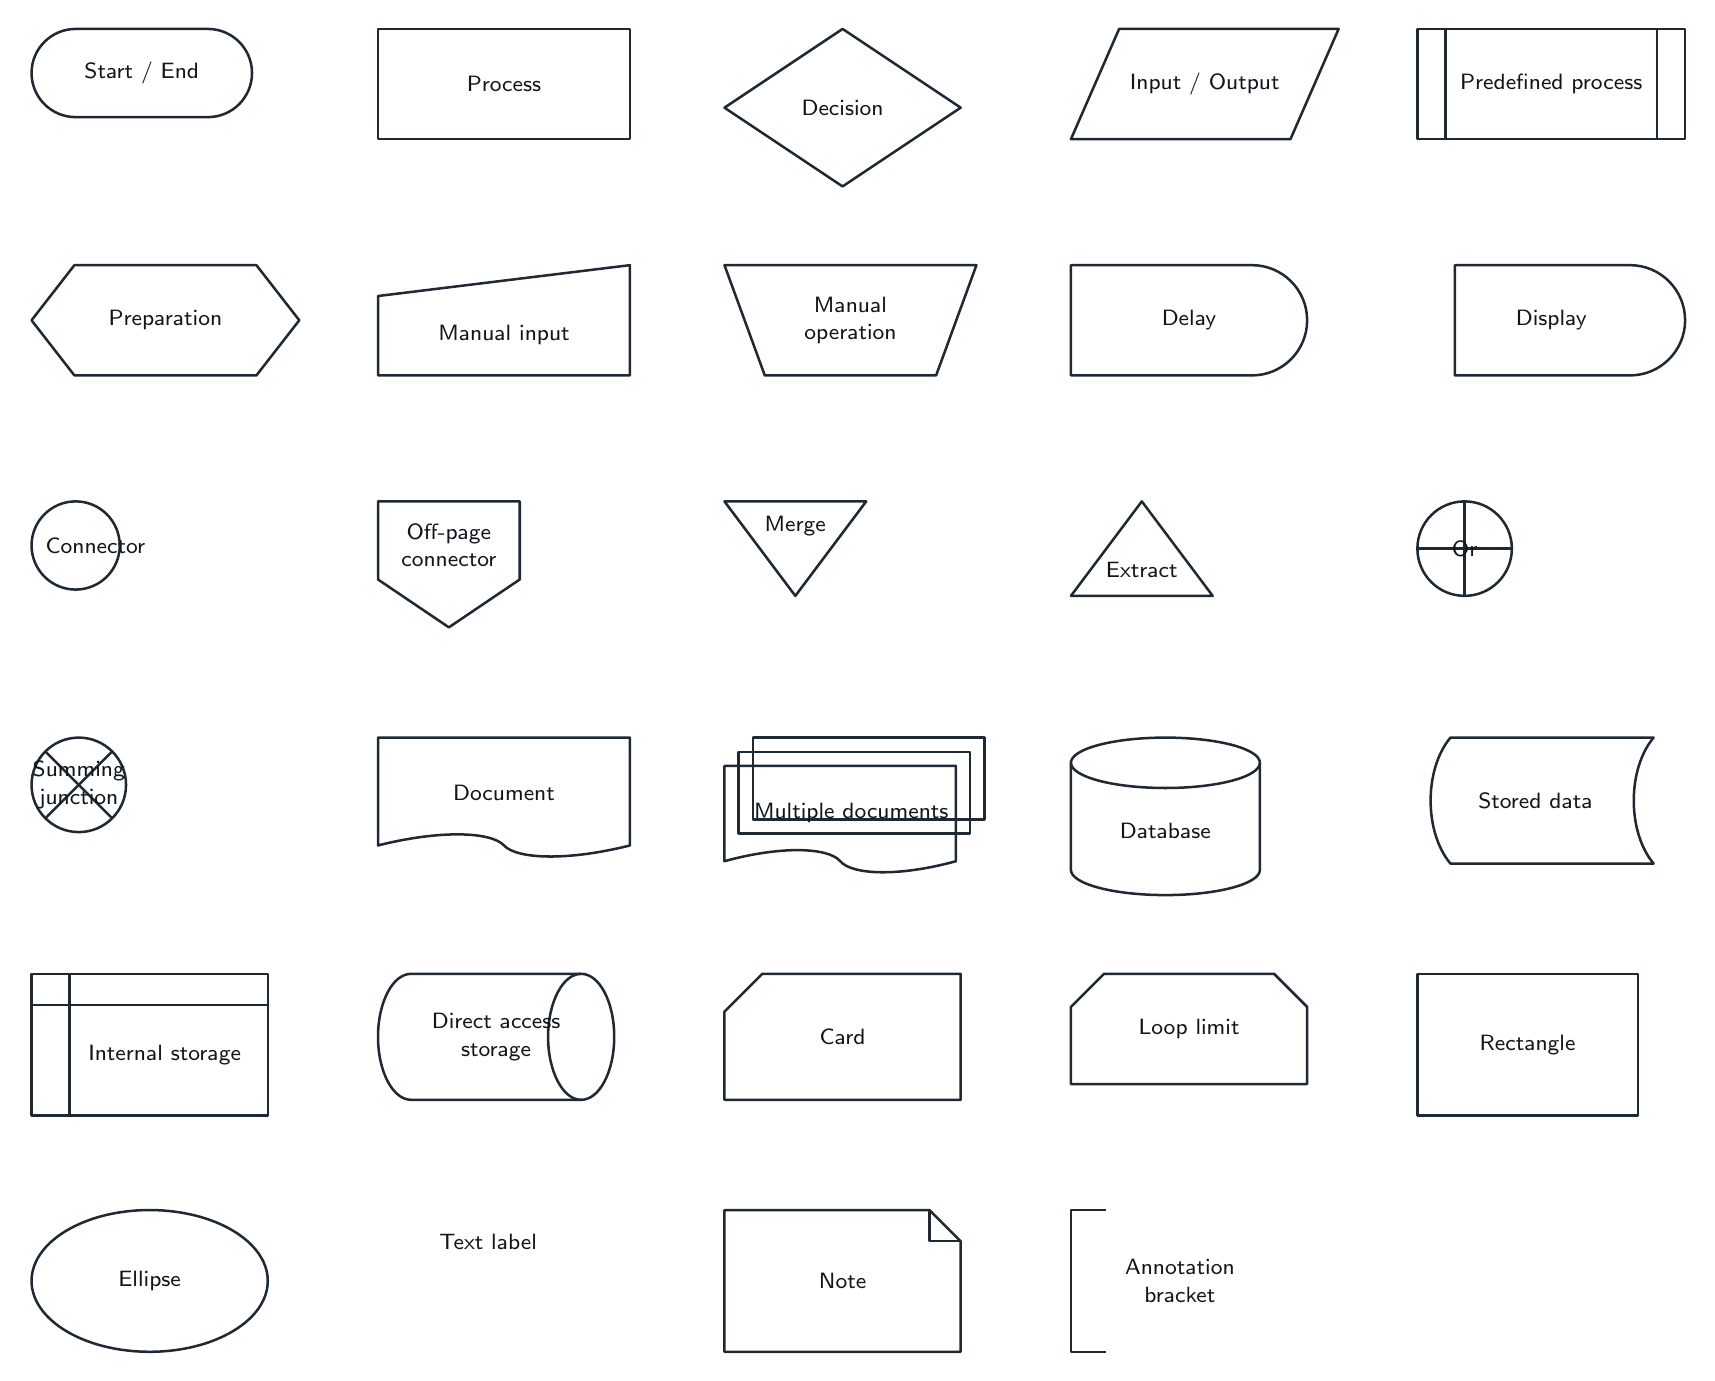
\begin{tikzpicture}[x=1cm, y=1cm]
  % ---- Nodes ----
  % n1 - Start / End "Start / End"
  \node[fcnode, shape=rounded rectangle, minimum width=2.8cm, minimum height=1.12cm,
        rounded rectangle arc length=180, draw=fc1F2933, line width=0.91pt, fill=white,
        font=\fontsize{7.97pt}{9.96pt}\selectfont\sffamily, text=fc12161C, align=center,
        text width=2.128cm] (n1) at (3.4,-2.56) {Start / End};
  % n2 - Process "Process"
  \node[fcnode, shape=rectangle, minimum width=3.2cm, minimum height=1.4cm, draw=fc1F2933,
        line width=0.91pt, fill=white, font=\fontsize{7.97pt}{9.96pt}\selectfont\sffamily,
        text=fc12161C, align=center, text width=2.88cm] (n2) at (8,-2.7) {Process};
  % n3 - Decision "Decision"
  \node[fcnode, shape=diamond, minimum width=3cm, minimum height=2cm, draw=fc1F2933,
        line width=0.91pt, fill=white, font=\fontsize{7.97pt}{9.96pt}\selectfont\sffamily,
        text=fc12161C, align=center, text width=1.5cm] (n3) at (12.3,-3) {Decision};
  % n4 - Input / Output "Input / Output"
  \draw[fcpath, draw=fc1F2933, line width=0.91pt, fill=white]
    (15.812,-2) -- (18.6,-2) -- (17.988,-3.4) -- (15.2,-3.4) -- cycle;
  \coordinate (n4) at (16.9,-2.7);
  \node[fclabel, anchor=center, font=\fontsize{7.97pt}{9.96pt}\selectfont\sffamily,
        text=fc12161C, align=center, text width=2.04cm] at (16.9,-2.7) {Input / Output};
  % n5 - Predefined process "Predefined process"
  \draw[fcpath, draw=fc1F2933, line width=0.91pt, fill=white]
    (19.6,-2) -- (23,-2) -- (23,-3.4) -- (19.6,-3.4) -- cycle;
  \draw[fcpath, draw=fc1F2933, line width=0.91pt]
    (19.96,-2) -- (19.96,-3.4);
  \draw[fcpath, draw=fc1F2933, line width=0.91pt]
    (22.64,-2) -- (22.64,-3.4);
  \coordinate (n5) at (21.3,-2.7);
  \node[fclabel, anchor=center, font=\fontsize{7.97pt}{9.96pt}\selectfont\sffamily,
        text=fc12161C, align=center, text width=2.52cm] at (21.3,-2.7) {Predefined process};
  % n6 - Preparation "Preparation"
  \draw[fcpath, draw=fc1F2933, line width=0.91pt, fill=white]
    (2.544,-5) -- (4.856,-5) -- (5.4,-5.7) -- (4.856,-6.4) -- (2.544,-6.4) -- (2,-5.7)
    -- cycle;
  \coordinate (n6) at (3.7,-5.7);
  \node[fclabel, anchor=center, font=\fontsize{7.97pt}{9.96pt}\selectfont\sffamily,
        text=fc12161C, align=center, text width=2.176cm] at (3.7,-5.7) {Preparation};
  % n7 - Manual input "Manual input"
  \draw[fcpath, draw=fc1F2933, line width=0.91pt, fill=white]
    (6.4,-5.392) -- (9.6,-5) -- (9.6,-6.4) -- (6.4,-6.4) -- cycle;
  \coordinate (n7) at (8,-5.7);
  \node[fclabel, anchor=center, font=\fontsize{7.97pt}{9.96pt}\selectfont\sffamily,
        text=fc12161C, align=center, text width=2.88cm] at (8,-5.882) {Manual input};
  % n8 - Manual operation "Manual operation"
  \draw[fcpath, draw=fc1F2933, line width=0.91pt, fill=white]
    (10.8,-5) -- (14,-5) -- (13.488,-6.4) -- (11.312,-6.4) -- cycle;
  \coordinate (n8) at (12.4,-5.7);
  \node[fclabel, anchor=center, font=\fontsize{7.97pt}{9.96pt}\selectfont\sffamily,
        text=fc12161C, align=center, text width=2.048cm] at (12.4,-5.7) {Manual operation};
  % n9 - Delay "Delay"
  \draw[fcpath, draw=fc1F2933, line width=0.91pt, fill=white]
    (15.2,-5) -- (17.5,-5) .. controls (17.8866,-5) and (18.2,-5.3134) .. (18.2,-5.7)
    .. controls (18.2,-6.0866) and (17.8866,-6.4) .. (17.5,-6.4) -- (15.2,-6.4) -- cycle;
  \coordinate (n9) at (16.7,-5.7);
  \node[fclabel, anchor=center, font=\fontsize{7.97pt}{9.96pt}\selectfont\sffamily,
        text=fc12161C, align=center, text width=2.6cm] at (16.7,-5.7) {Delay};
  % n10 - Display "Display"
  \draw[fcpath, draw=fc1F2933, line width=0.91pt, fill=white]
    (20.076,-5) -- (22.3,-5) .. controls (22.6866,-5) and (23,-5.3134) .. (23,-5.7)
    .. controls (23,-6.0866) and (22.6866,-6.4) .. (22.3,-6.4) -- (20.076,-6.4) -- cycle;
  \coordinate (n10) at (21.3,-5.7);
  \node[fclabel, anchor=center, font=\fontsize{7.97pt}{9.96pt}\selectfont\sffamily,
        text=fc12161C, align=center, text width=2.312cm] at (21.3,-5.7) {Display};
  % n11 - Connector "Connector"
  \node[fcnode, shape=circle, minimum size=1.12cm, draw=fc1F2933, line width=0.91pt,
        fill=white, font=\fontsize{7.97pt}{9.96pt}\selectfont\sffamily, text=fc12161C,
        align=center, text width=0.7616cm] (n11) at (2.56,-8.56) {Connector};
  % n12 - Off-page connector "Off-page connector"
  \draw[fcpath, draw=fc1F2933, line width=0.91pt, fill=white]
    (6.4,-8) -- (8.2,-8) -- (8.2,-8.992) -- (7.3,-9.6) -- (6.4,-8.992) -- cycle;
  \coordinate (n12) at (7.3,-8.8);
  \node[fclabel, anchor=center, font=\fontsize{7.97pt}{9.96pt}\selectfont\sffamily,
        text=fc12161C, align=center, text width=1.56cm] at (7.3,-8.56) {Off-page connector};
  % n13 - Merge "Merge"
  \draw[fcpath, draw=fc1F2933, line width=0.91pt, fill=white]
    (10.8,-8) -- (12.6,-8) -- (11.7,-9.2) -- cycle;
  \coordinate (n13) at (11.7,-8.6);
  \node[fclabel, anchor=center, font=\fontsize{7.97pt}{9.96pt}\selectfont\sffamily,
        text=fc12161C, align=center, text width=1.08cm] at (11.7,-8.31) {Merge};
  % n14 - Extract "Extract"
  \draw[fcpath, draw=fc1F2933, line width=0.91pt, fill=white]
    (16.1,-8) -- (17,-9.2) -- (15.2,-9.2) -- cycle;
  \coordinate (n14) at (16.1,-8.6);
  \node[fclabel, anchor=center, font=\fontsize{7.97pt}{9.96pt}\selectfont\sffamily,
        text=fc12161C, align=center, text width=1.08cm] at (16.1,-8.87) {Extract};
  % n15 - Or "Or"
  \draw[fcpath, draw=fc1F2933, line width=0.91pt, fill=white]
    (20.2,-8) .. controls (20.5314,-8) and (20.8,-8.2686) .. (20.8,-8.6)
    .. controls (20.8,-8.9314) and (20.5314,-9.2) .. (20.2,-9.2)
    .. controls (19.8686,-9.2) and (19.6,-8.9314) .. (19.6,-8.6)
    .. controls (19.6,-8.2686) and (19.8686,-8) .. (20.2,-8) -- cycle;
  \draw[fcpath, draw=fc1F2933, line width=0.91pt]
    (19.6,-8.6) -- (20.8,-8.6);
  \draw[fcpath, draw=fc1F2933, line width=0.91pt]
    (20.2,-8) -- (20.2,-9.2);
  \coordinate (n15) at (20.2,-8.6);
  \node[fclabel, anchor=center, font=\fontsize{7.97pt}{9.96pt}\selectfont\sffamily,
        text=fc12161C, align=center, text width=1.2cm] at (20.2,-8.6) {Or};
  % n16 - Summing junction "Summing junction"
  \draw[fcpath, draw=fc1F2933, line width=0.91pt, fill=white]
    (2.6,-11) .. controls (2.9314,-11) and (3.2,-11.2686) .. (3.2,-11.6)
    .. controls (3.2,-11.9314) and (2.9314,-12.2) .. (2.6,-12.2)
    .. controls (2.2686,-12.2) and (2,-11.9314) .. (2,-11.6)
    .. controls (2,-11.2686) and (2.2686,-11) .. (2.6,-11) -- cycle;
  \draw[fcpath, draw=fc1F2933, line width=0.91pt]
    (2.1757,-11.1757) -- (3.0243,-12.0243);
  \draw[fcpath, draw=fc1F2933, line width=0.91pt]
    (3.0243,-11.1757) -- (2.1757,-12.0243);
  \coordinate (n16) at (2.6,-11.6);
  \node[fclabel, anchor=center, font=\fontsize{7.97pt}{9.96pt}\selectfont\sffamily,
        text=fc12161C, align=center, text width=1.2cm] at (2.6,-11.6) {Summing junction};
  % n17 - Document "Document"
  \draw[fcpath, draw=fc1F2933, line width=0.91pt, fill=white]
    (6.4,-11) -- (9.6,-11) -- (9.6,-12.3696)
    .. controls (8.8,-12.5712) and (8.16,-12.5424) .. (8,-12.3696)
    .. controls (7.84,-12.1968) and (7.2,-12.168) .. (6.4,-12.3696) -- cycle;
  \coordinate (n17) at (8,-11.8);
  \node[fclabel, anchor=center, font=\fontsize{7.97pt}{9.96pt}\selectfont\sffamily,
        text=fc12161C, align=center, text width=2.88cm] at (8,-11.696) {Document};
  % n18 - Multiple documents "Multiple documents"
  \draw[fcpath, draw=fc1F2933, line width=0.91pt, fill=white]
    (10.8,-11.36) -- (13.74,-11.36) -- (13.74,-12.5696)
    .. controls (13.005,-12.7712) and (12.417,-12.7424) .. (12.27,-12.5696)
    .. controls (12.123,-12.3968) and (11.535,-12.368) .. (10.8,-12.5696) -- cycle;
  \draw[fcpath, draw=fc1F2933, line width=0.91pt]
    (11.16,-11) -- (14.1,-11) -- (14.1,-12.0368) -- (11.16,-12.0368) -- cycle;
  \draw[fcpath, draw=fc1F2933, line width=0.91pt]
    (10.98,-11.18) -- (13.92,-11.18) -- (13.92,-12.2168) -- (10.98,-12.2168) -- cycle;
  \coordinate (n18) at (12.45,-11.9);
  \node[fclabel, anchor=center, font=\fontsize{7.97pt}{9.96pt}\selectfont\sffamily,
        text=fc12161C, align=center, text width=2.82cm]
        at (12.41,-11.954) {Multiple documents};
  % n19 - Database "Database"
  \draw[fcpath, draw=fc1F2933, line width=0.91pt, fill=white]
    (15.2,-11.32) .. controls (15.2,-11.1433) and (15.7372,-11) .. (16.4,-11)
    .. controls (17.0628,-11) and (17.6,-11.1433) .. (17.6,-11.32) -- (17.6,-12.68)
    .. controls (17.6,-12.8567) and (17.0628,-13) .. (16.4,-13)
    .. controls (15.7372,-13) and (15.2,-12.8567) .. (15.2,-12.68) -- cycle;
  \draw[fcpath, draw=fc1F2933, line width=0.91pt]
    (15.2,-11.32) .. controls (15.2,-11.4967) and (15.7372,-11.64) .. (16.4,-11.64)
    .. controls (17.0628,-11.64) and (17.6,-11.4967) .. (17.6,-11.32);
  \coordinate (n19) at (16.4,-12);
  \node[fclabel, anchor=center, font=\fontsize{7.97pt}{9.96pt}\selectfont\sffamily,
        text=fc12161C, align=center, text width=2.08cm] at (16.4,-12.18) {Database};
  % n20 - Stored data "Stored data"
  \draw[fcpath, draw=fc1F2933, line width=0.91pt, fill=white]
    (20.02,-11) -- (22.6,-11) .. controls (22.264,-11.4) and (22.264,-12.2) .. (22.6,-12.6)
    -- (20.02,-12.6) .. controls (19.684,-12.2) and (19.684,-11.4) .. (20.02,-11) -- cycle;
  \coordinate (n20) at (21.1,-11.8);
  \node[fclabel, anchor=center, font=\fontsize{7.97pt}{9.96pt}\selectfont\sffamily,
        text=fc12161C, align=center, text width=2.04cm] at (21.1,-11.8) {Stored data};
  % n21 - Internal storage "Internal storage"
  \draw[fcpath, draw=fc1F2933, line width=0.91pt, fill=white]
    (2,-14) -- (5,-14) -- (5,-15.8) -- (2,-15.8) -- cycle;
  \draw[fcpath, draw=fc1F2933, line width=0.91pt]
    (2.48,-14) -- (2.48,-15.8);
  \draw[fcpath, draw=fc1F2933, line width=0.91pt]
    (2,-14.396) -- (5,-14.396);
  \coordinate (n21) at (3.5,-14.9);
  \node[fclabel, anchor=center, font=\fontsize{7.97pt}{9.96pt}\selectfont\sffamily,
        text=fc12161C, align=center, text width=2.3cm] at (3.69,-15.036) {Internal storage};
  % n22 - Direct access storage "Direct access storage"
  \draw[fcpath, draw=fc1F2933, line width=0.91pt, fill=white]
    (6.82,-14) -- (8.98,-14) .. controls (9.212,-14) and (9.4,-14.3582) .. (9.4,-14.8)
    .. controls (9.4,-15.2418) and (9.212,-15.6) .. (8.98,-15.6) -- (6.82,-15.6)
    .. controls (6.588,-15.6) and (6.4,-15.2418) .. (6.4,-14.8)
    .. controls (6.4,-14.3582) and (6.588,-14) .. (6.82,-14) -- cycle;
  \draw[fcpath, draw=fc1F2933, line width=0.91pt]
    (8.98,-14) .. controls (8.748,-14) and (8.56,-14.3582) .. (8.56,-14.8)
    .. controls (8.56,-15.2418) and (8.748,-15.6) .. (8.98,-15.6);
  \coordinate (n22) at (7.9,-14.8);
  \node[fclabel, anchor=center, font=\fontsize{7.97pt}{9.96pt}\selectfont\sffamily,
        text=fc12161C, align=center, text width=2.04cm]
        at (7.9,-14.8) {Direct access storage};
  % n23 - Card "Card"
  \draw[fcpath, draw=fc1F2933, line width=0.91pt, fill=white]
    (11.28,-14) -- (13.8,-14) -- (13.8,-15.6) -- (10.8,-15.6) -- (10.8,-14.48) -- cycle;
  \coordinate (n23) at (12.3,-14.8);
  \node[fclabel, anchor=center, font=\fontsize{7.97pt}{9.96pt}\selectfont\sffamily,
        text=fc12161C, align=center, text width=2.6cm] at (12.3,-14.8) {Card};
  % n24 - Loop limit "Loop limit"
  \draw[fcpath, draw=fc1F2933, line width=0.91pt, fill=white]
    (15.62,-14) -- (17.78,-14) -- (18.2,-14.42) -- (18.2,-15.4) -- (15.2,-15.4)
    -- (15.2,-14.42) -- cycle;
  \coordinate (n24) at (16.7,-14.7);
  \node[fclabel, anchor=center, font=\fontsize{7.97pt}{9.96pt}\selectfont\sffamily,
        text=fc12161C, align=center, text width=2.6cm] at (16.7,-14.7) {Loop limit};
  % n25 - Rectangle "Rectangle"
  \node[fcnode, shape=rectangle, minimum width=2.8cm, minimum height=1.8cm, draw=fc1F2933,
        line width=0.91pt, fill=white, font=\fontsize{7.97pt}{9.96pt}\selectfont\sffamily,
        text=fc12161C, align=center, text width=2.48cm] (n25) at (21,-14.9) {Rectangle};
  % n26 - Ellipse "Ellipse"
  \node[fcnode, shape=ellipse, minimum width=3cm, minimum height=1.8cm, draw=fc1F2933,
        line width=0.91pt, fill=white, font=\fontsize{7.97pt}{9.96pt}\selectfont\sffamily,
        text=fc12161C, align=center, text width=2.04cm] (n26) at (3.5,-17.9) {Ellipse};
  % n27 - Text label "Text label"
  \node[fclabel, anchor=center, font=\fontsize{7.97pt}{9.96pt}\selectfont\sffamily,
        text=fc12161C, align=center, text width=2.8cm] (n27) at (7.8,-17.4) {Text label};
  % n28 - Note "Note"
  \draw[fcpath, draw=fc1F2933, line width=0.91pt, fill=white]
    (10.8,-17) -- (13.404,-17) -- (13.8,-17.396) -- (13.8,-18.8) -- (10.8,-18.8) -- cycle;
  \draw[fcpath, draw=fc1F2933, line width=0.91pt]
    (13.404,-17) -- (13.404,-17.396) -- (13.8,-17.396);
  \coordinate (n28) at (12.3,-17.9);
  \node[fclabel, anchor=center, font=\fontsize{7.97pt}{9.96pt}\selectfont\sffamily,
        text=fc12161C, align=center, text width=2.6cm] at (12.3,-17.9) {Note};
  % n29 - Annotation bracket "Annotation bracket"
  \draw[fcpath, draw=fc1F2933, line width=0.91pt]
    (15.64,-17) -- (15.2,-17) -- (15.2,-18.8) -- (15.64,-18.8);
  \coordinate (n29) at (16.4,-17.9);
  \node[fclabel, anchor=center, font=\fontsize{7.97pt}{9.96pt}\selectfont\sffamily,
        text=fc12161C, align=center, text width=1.728cm]
        at (16.584,-17.9) {Annotation bracket};
\end{tikzpicture}
\end{document}